\section{ER Diagram}
The ER diagram describes the entities and their individual relations. The group based the current diagram on last year's, re-using some attributes for entities, but cleaning up relations and adding new content needed by other groups (e.g. pictogram category). The central entities are the profile, the applications available to that profile and the pictograms linked to it.%TODO:ref earlier report here

The profile holds information about the user, such as name, phone number, picture, e-mail, address and their role (e.g. parent or department employee). Roles are important in determining the privileges of the account. The pictograms available to the profile are selected by the guardians, in the case of a child.

The settings of an application are saved in the link to the profile in order to allow diffrerent users to costumize the look of the application.

The fact that applications and pictograms can be linked to department signifies, that a department can allow all users affiliated with it to have access to specific applications and pictograms related to that department.

\begin{figure}[h]
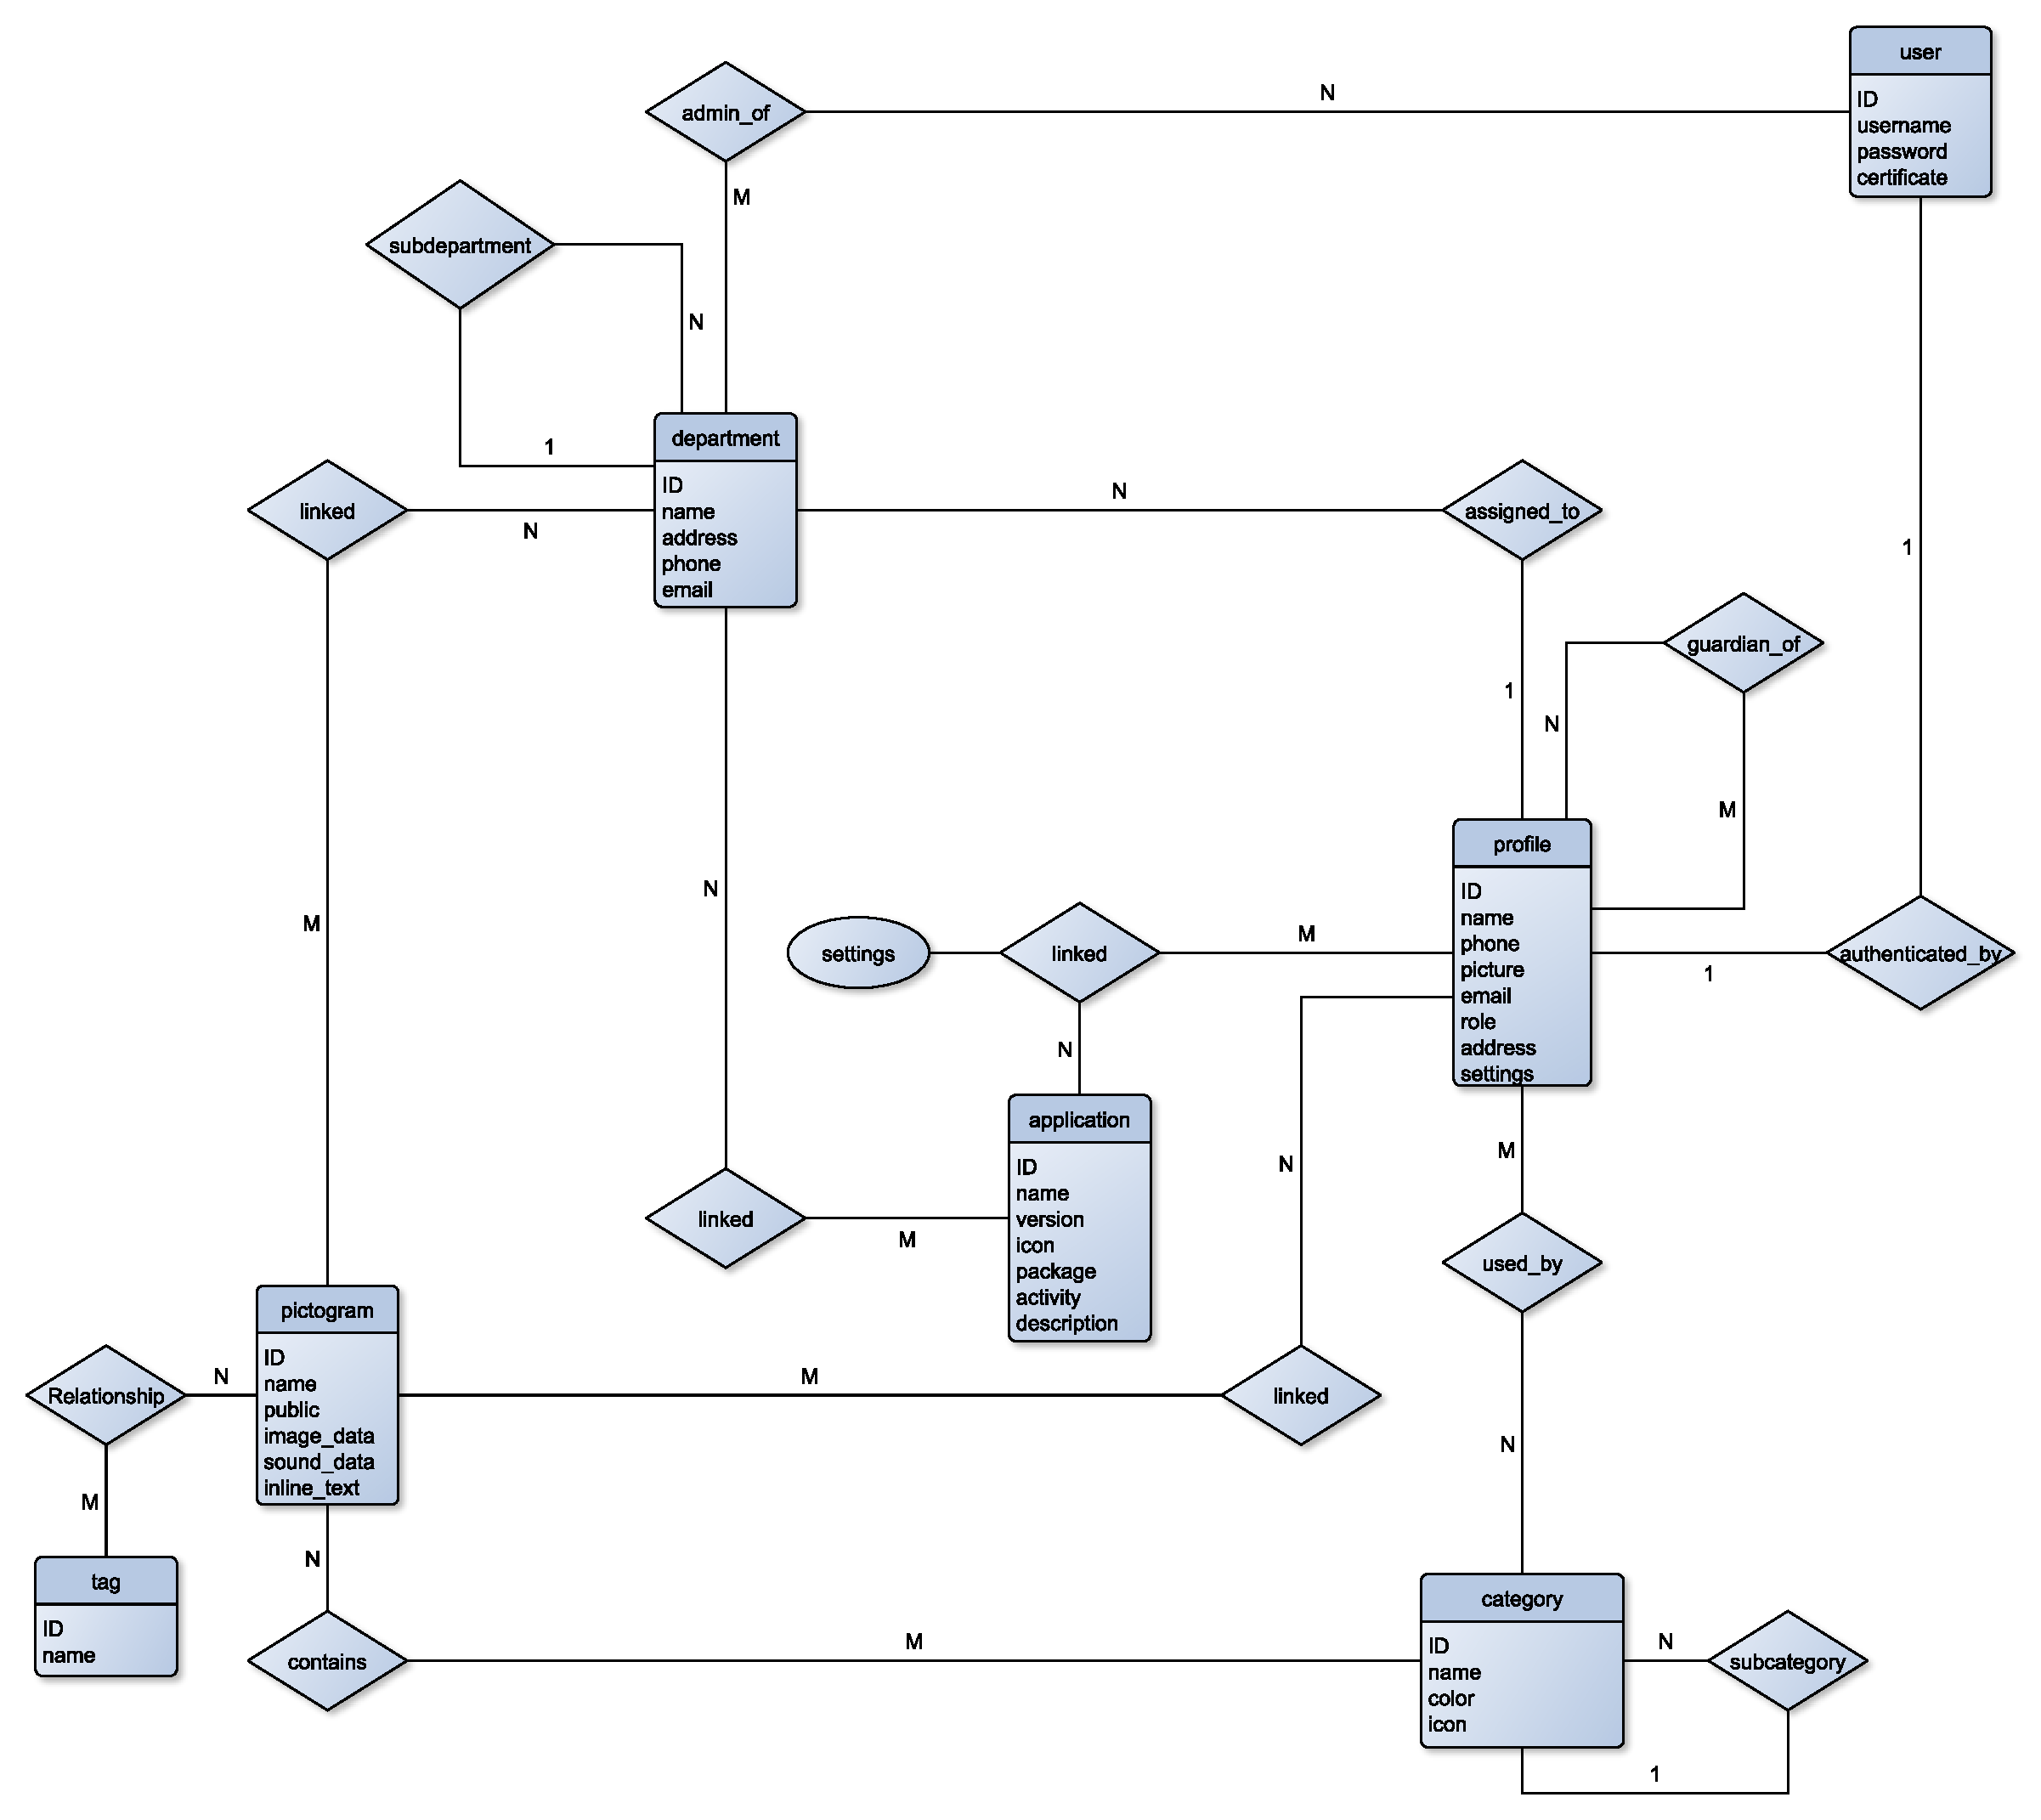
\includegraphics[width=\textwidth]{img/ER_diagram.pdf}
\label{fig:erdiagram}
\caption{ER Diagram}
\end{figure}